\documentclass[../../../main.tex]{subfiles}
\begin{document}

In the field of metal additive manufacturing, various technologies offer distinct material deposition and fusion strategies, each with its own advantages and limitations in terms of cost, precision, and resulting mechanical properties. 
Among the most established is selective laser melting (SLM/DMLS), in which a high-power laser beam melts metal powder in a localised manner, layer by layer, on a powder bed. 
This technique enables the production of parts with complex geometries and very high density, comparable to that of forged material. 
However, it has drawbacks associated with the high cost of the process, the need for supports and heat treatments, as well as the occurrence of residual stresses.

Faced with these limitations, direct deposition technologies such as WAAM (Wire Arc Additive Manufacturing) or DED (Directed Energy Deposition) offer alternatives based on the direct fusion of wire or metal powder using an electric arc or laser. 
In the case of WAAM, the great advantage lies in the low cost of the process and high productivity, making it an interesting option for large components. 
In addition, the parts obtained tend to have mechanical properties, particularly fatigue properties, that exceed those manufactured with SLM/DMLS.
However, surface quality is limited, geometric accuracy is reduced, and, in the case of complex lattice structures, there is uncertainty as to whether the technology could adequately reproduce the desired geometry. 
An additional motivation for considering WAAM was the possibility of non-planar printing, taking advantage of a previously developed G-Code trajectory generation module, which opened up an additional field of exploration in additive manufacturing beyond the conventional flat layer scheme.
Due to the complexity of the geometry, a 6-axis machine would be required to print the structure using WAAM. 
The number of companies that have this type of machine is limited, as WAAM technology is not widely used. 
Several companies based in the author's country that have this technology were contacted, but no positive response to collaborate was received.

After a search for international partners, the French company Tetmet SAS\footnote{\href{https://www.tetmet.net/}{Tetmet}.} (La Défense, France) was discovered. 
Tetmet proposes a disruptive alternative through its process called ASLM (Adaptive Spatial Lattice Manufacturing). 
Unlike traditional additive manufacturing techniques, ASLM is not based on layer-by-layer deposition, but rather on the construction of lattice structures from metal rods assembled and joined by robotically controlled spot laser welding. 
This strategy eliminates the stratification characteristic of conventional 3D printing, which should translate into increased structural strength by avoiding layer interfaces that are often weak points under dynamic or fatigue loads. 
In addition, the process is significantly more economical than SLM or WAAM, and allows for the exploration of new possibilities in the generation of optimised, lightweight and resistant spatial structures.

Consequently, although the option of manufacturing the support using DMLS was initially considered, and WAAM was subsequently considered due to its greater mechanical robustness and lower cost, it was finally decided to opt for Tetmet's technology. 
This choice was made for several reasons: the interest in exploring the potential of an emerging process with a completely different manufacturing strategy, the expectation of obtaining improved strength thanks to the elimination of layers and, very importantly, the possibility of further reducing production costs without compromising structural functionality.

Due to budget constraints, it was not possible to manufacture the entire bracket, so it was decided to manufacture only half of it. 
The size of the bars used was 1.6 \textit{mm}, and the material used was steel.
A base plate made of the same material was used to manufacture the piece, so the horizontal edges of the base had to be removed. 
In addition, Tetmet reconditioned the lattice by removing certain edges close to each other to facilitate manufacturing.
The total weight of the result part is 1588 \textit{g}.
\cref{fig:fab_1} shows some images of the manufacturing process, and \cref{fig:fab_2} shows some images of the final result of the manufacturing process.

\begin{figure}[!htbp]
    \centering
    \begin{subfigure}[b]{0.45\textwidth}
        \includegraphics[width = \textwidth]{imgs/img_1.jpg}
     \end{subfigure}
     \hspace{3em}
    \begin{subfigure}[b]{0.45\textwidth}
        \includegraphics[width =\textwidth]{imgs/img_4.jpg}
     \end{subfigure}
     \caption{Images of the manufacturing process using ASML}
    \label{fig:fab_1}
\end{figure}


Although part of the adapter could be manufactured, the chosen manufacturing method is still a new one that needs to be refined, especially in terms of the strategy for joining the edges at the nodes. 
\cref{fig:fab_3} shows some details of the nodes where the poor quality of the joints can be seen. 
In addition, during the manufacturer's structural modification to facilitate manufacturing, edges were removed, leaving some isolated. 
Despite this, the structure was printed as agreed with the manufacturer at a considerably lower price than any other metal 3D printing method. 
However, the manufacturing time was two weeks. 
It is worth mentioning that Tetmet is constantly working to improve manufacturing times, and this was the first case of a random lattice structure they had ever worked on. 
As it was not possible to manufacture the entire part, mechanical and vibration tests were not carried out to validate the part. Therefore, the manufactured part is left as proof of concept and analysis of ASLM technology.

\begin{figure}[!htbp]
    \centering
    \begin{subfigure}[b]{0.8\textwidth}
        \includegraphics[width = \textwidth]{imgs/img_2.jpg}
     \end{subfigure}
     \vspace{1cm}
    \begin{subfigure}[b]{0.8\textwidth}
        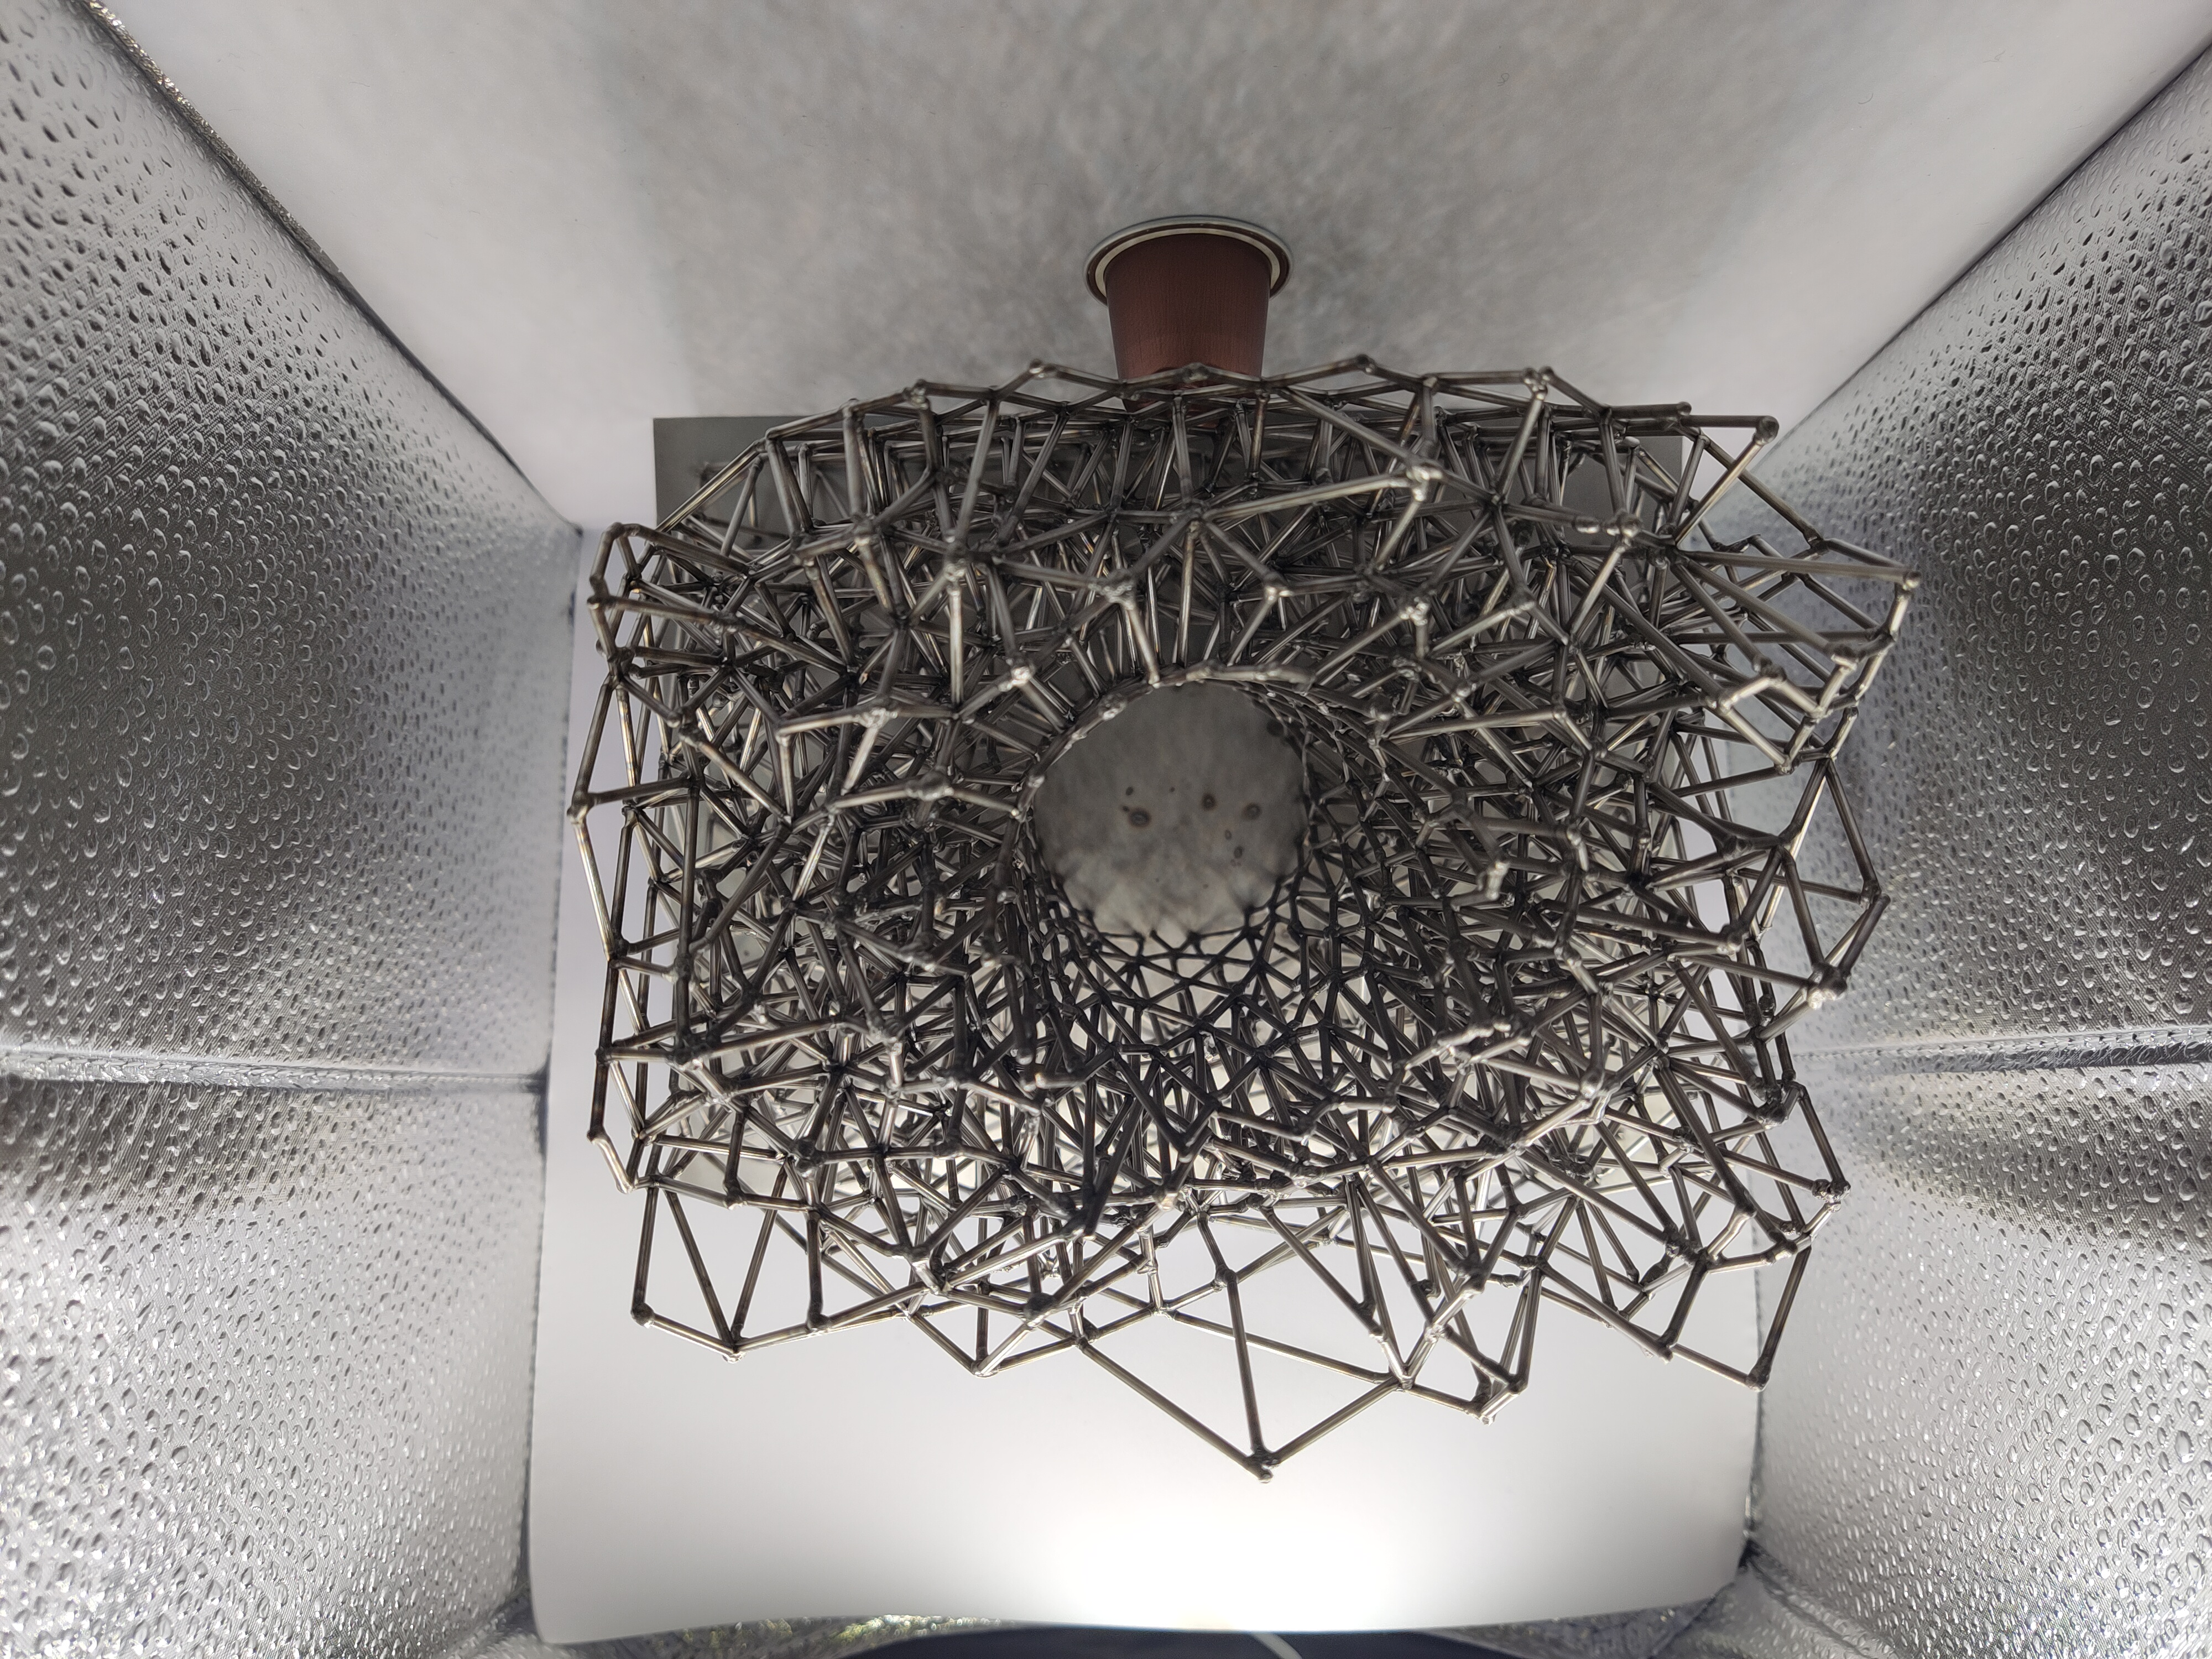
\includegraphics[width =\textwidth, angle=180]{imgs/img_3.jpg}
     \end{subfigure}
     \caption{Result of the manufacturing process for half of the bracket's body using ASML.}
    \label{fig:fab_2}
\end{figure}

\begin{figure}[!htbp]
    \centering
    \begin{subfigure}[b]{0.35\textwidth}
        \includegraphics[width = \textwidth]{imgs/node1.jpg}
     \end{subfigure}
     \vspace{0.5cm}
     \hspace{0.3cm}
    \begin{subfigure}[b]{0.35\textwidth}
        \includegraphics[width =\textwidth]{imgs/node2.jpg}
     \end{subfigure}
         \begin{subfigure}[b]{0.35\textwidth}
        \includegraphics[width =\textwidth]{imgs/node3.jpg}
     \end{subfigure}
     \hspace{0.3cm}
    \begin{subfigure}[b]{0.35\textwidth}
        \includegraphics[width =\textwidth]{imgs/node4.jpg}
     \end{subfigure}
     \caption{Details of certain nodes of the final manufactured structure.}
    \label{fig:fab_3}
\end{figure}

\end{document}